\documentclass[11pt]{article}
\usepackage[T1]{fontenc}
\usepackage[utf8]{inputenc}
\usepackage{lmodern,microtype}
\usepackage[margin=1in]{geometry}
\usepackage{amsmath,amssymb,bm}
\usepackage{graphicx,booktabs}
\usepackage[numbers,sort&compress]{natbib}
\usepackage{xcolor}
\usepackage[colorlinks=true,linkcolor=blue!50!black,citecolor=blue!50!black,urlcolor=blue!50!black]{hyperref}
\usepackage{tikz}
\usetikzlibrary{arrows.meta,positioning,fit,calc}
\usepackage{caption}
\captionsetup{font=small,labelfont=bf}

\newcommand{\jev}{Jev}
\newcommand{\PH}[1]{\textcolor{red}{[#1]}}
\newcommand{\Eh}{\ensuremath{\mathrm{m}E_h}}

\title{Is there a Hamiltonian inside a decision model?\\ Probing the energy landscape of \jev{} for quantum chemistry}
\author{Eric Dong\\ Independent researcher\\ \texttt{dongzhaohe321418@gmail.com}}
\date{}

\begin{document}
\maketitle

\begin{abstract}
\jev{} is a proprietary ``System One'' model that returns calibrated probability distributions over a fixed, typed answer schema instead of text, and answers many questions about one input in a single parallel pass.
Any such output defines local energies $E=-\log p$, so it is natural to ask whether these energies form one Hamiltonian-like landscape and whether that landscape is useful for quantum chemistry.
We test this through black-box access to \texttt{jev-1.13.0} with 2,235 distinct queries, using PySCF for ground truth.
The conditionals are close to, but not exactly, those of a single joint distribution: the logically forced coupling is symmetric, yet 57\% of inferred pairwise couplings are asymmetric beyond three bootstrap standard errors, and complementary statements do not sum to one.
Given a Hamiltonian written in the prompt, \jev{} does not track its spectrum. Its preferences over Ising configurations follow the signs of the printed coefficients, so rewriting the same energies in the textbook sign convention reverses the rank correlation (from $-0.41$ to $+0.34$ for four spins), and its energy read-out for H$_2$ is off by 104~\Eh{} on average.
On quantum-chemistry decisions it ranks multireference character, $T_1$ diagnostics and RHF instability with AUROC 0.74--0.89, comparable to a two-feature logistic model, but it is poorly calibrated and falls to 0.60--0.68 when the molecule's name is removed.
As an importance prior for selected configuration interaction it beats random selection in all ten systems and loses to a first-order perturbative estimate in nine.
\jev{} therefore behaves as a fast triage layer driven by textual cues, and its outputs should not be read as a physical energy landscape.
\end{abstract}

\section{Introduction}

A classifier that outputs a probability distribution $p(y\mid x)$ can always be rewritten as a Gibbs distribution $p(y\mid x)\propto \exp[-E(x,y)]$ with $E=-\log p$ up to a constant \citep{lecun2006tutorial,grathwohl2019your}.
For one softmax head the rewriting says nothing new.
It says more when a model answers \emph{several} questions about the same input, because the per-question energies may or may not assemble into one landscape over joint answers, as the conditionals of a Boltzmann machine do \citep{ackley1985learning}.
Only a single landscape can be sampled, minimised or added to a physical Hamiltonian, the uses that Ising and QUBO encodings make routine \citep{lucas2014ising,kadowaki1998quantum}.

\jev{} \citep{typesafe2026introducing,typesafe2026api} makes this question concrete.
It accepts text or structured state and a set of typed questions (a yes/no \emph{Noul}, a \emph{Choice} over at most 255 options, or a \emph{Score} over 2--10 ordered levels) and returns a probability for every allowed answer, trained, according to its developer, for calibration against outcomes rather than for human preference.
Questions are evaluated in parallel, latency is well under a second, and outputs cannot fall outside the schema \citep{willison2026jev}.
A quantum-chemistry workflow makes many small typed decisions of this kind before any expensive calculation: is the system multireference, which spin state is lowest, which determinants matter.
The developer also warns that structural invariants ``aren't guaranteed'' and that the model ``is not a calculator'' \citep{typesafe2026jaggedness}.

We ask three questions and answer each with measurements.
(i)~Do \jev{}'s conditionals admit a single joint landscape?
We test coupling symmetry and total probability, the classical compatibility conditions for conditionals \citep{besag1974spatial,arnold1989compatible}, against a coherent null matched to \jev{}'s own noise, with a positive control in which the exact joint is written in the input.
(ii)~Does \jev{} represent a Hamiltonian written into its input?
We give it random Ising models and the Jordan--Wigner qubit Hamiltonian of H$_2$ \citep{jordan1928pauli,omalley2016scalable}, and change only how they are written.
(iii)~Is it useful for quantum-chemistry decisions?
We score its predictions of multireference diagnostics against PySCF labels with proper scoring rules \citep{gneiting2007strictly}, ablate its inputs, and use it to rank determinants for selected configuration interaction \citep{huron1973iterative,holmes2016heat}.
\PH{E5-E7 sentence.}
Figure~\ref{fig:overview} summarises the design.

We find that \jev{}'s local energies contain an approximate pairwise landscape with predictive value but are measurably incoherent, that its reading of a Hamiltonian follows printed signs and textbook recall rather than energies, and that its chemistry skill mostly reflects a stretch factor stated in the prompt.
The coherence tests need only black-box access and apply to any model that answers many questions about one input.
Code, cached API responses, referee reports and figures are released.

\begin{figure}[t]
\centering\hyphenpenalty=10000\exhyphenpenalty=10000
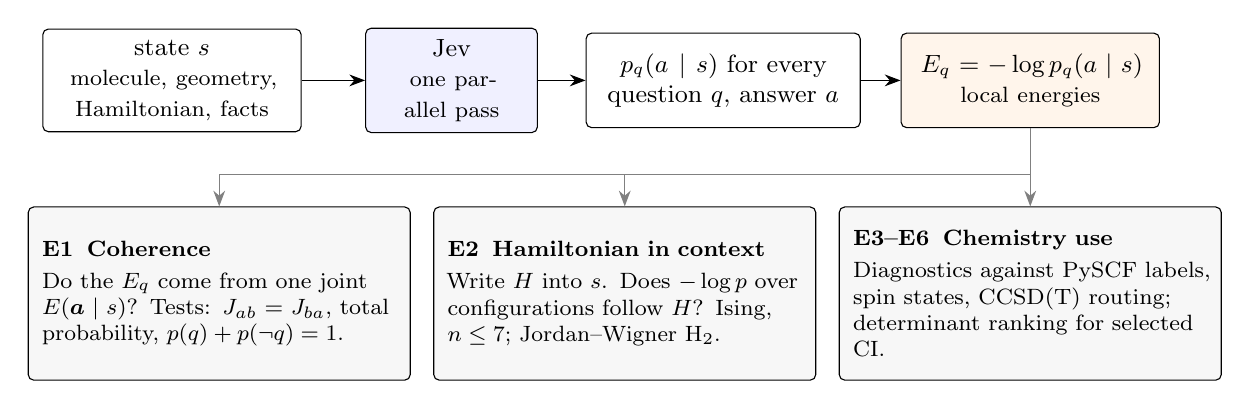
\begin{tikzpicture}[
  font=\small, >={Stealth[length=2mm]},
  box/.style={draw, rounded corners=2pt, align=center, inner sep=4pt, minimum height=12mm},
  probe/.style={draw, rounded corners=2pt, inner sep=5pt, text width=4.5cm, minimum height=22mm, fill=black!3,
                font=\footnotesize, align=left, anchor=north}]
\node[box, text width=3.0cm] (s) at (0,0) {state $s$\\{\footnotesize molecule, geometry,}\\{\footnotesize Hamiltonian, facts}};
\node[box, text width=1.9cm, fill=blue!6] (j) at (3.55,0) {\jev{}\\{\footnotesize one parallel pass}};
\node[box, text width=3.2cm] (p) at (7.0,0) {$p_q(a\mid s)$ for every\\question $q$, answer $a$};
\node[box, text width=3.0cm, fill=orange!8] (e) at (10.9,0) {$E_q=-\log p_q(a\mid s)$\\{\footnotesize local energies}};
\draw[->] (s) -- (j); \draw[->] (j) -- (p); \draw[->] (p) -- (e);
\node[probe] (p1) at (0.6,-1.6) {\textbf{E1\enspace Coherence}\\[2pt] Do the $E_q$ come from one joint $E(\bm a\mid s)$? Tests: $J_{ab}=J_{ba}$, total probability, $p(q)+p(\neg q)=1$.};
\node[probe] (p2) at (5.75,-1.6) {\textbf{E2\enspace Hamiltonian in context}\\[2pt] Write $H$ into $s$. Does $-\log p$ over configurations follow $H$? Ising, $n\le 7$; Jordan--Wigner H$_2$.};
\node[probe] (p3) at (10.9,-1.6) {\textbf{E3--E6\enspace Chemistry use}\\[2pt] Diagnostics against PySCF labels, spin states, CCSD(T) routing; determinant ranking for selected CI.};
\coordinate (bus) at (0,-1.2);
\draw[black!50] (e.south) |- (p1.north |- bus) ;
\foreach \t in {p1,p2,p3} \draw[->, black!50] (\t.north |- bus) -- (\t.north);
\end{tikzpicture}
\caption{Study design. \jev{} maps a state and a set of typed questions to answer distributions in one pass. Reading each distribution as a local energy, we test whether the local energies are consistent with one landscape (E1), whether they reproduce a Hamiltonian supplied in the input (E2), and whether they are useful for quantum-chemistry decisions (E3--E6). E7 repeats E1 and E2 on open-weight language models.}
\label{fig:overview}
\end{figure}

\section{Background and related work}

\paragraph{Classifiers as energy models.}
Energy-based models assign a scalar energy to each configuration and convert it to probability through a Gibbs distribution \citep{lecun2006tutorial}.
Hopfield networks and Boltzmann machines give such energies pairwise, symmetric couplings \citep{hopfield1982neural,ackley1985learning}, and attention can be read as the update of a continuous Hopfield energy \citep{ramsauer2020hopfield}.
\citet{grathwohl2019your} showed that the logits of any softmax classifier define a joint energy over inputs and labels, and \citet{winer2025deep} studied a random network as a Hamiltonian over its inputs.
These works treat one output head; \jev{} exposes many typed heads over one shared state, which is the setting where a joint landscape can fail to exist.

\paragraph{When do conditionals have a joint?}
Local conditional specifications define a joint distribution only under compatibility conditions \citep{besag1974spatial,hammersley1971markov,arnold1989compatible}.
Separately learned conditionals, as in dependency networks, are generally incompatible \citep{heckerman2000dependency}.
For binary variables compatibility has a simple necessary consequence: the log odds ratio between two variables is symmetric, so the coupling inferred from $b$'s effect on $a$ must equal that inferred from $a$'s effect on $b$.
Recent work finds logical incoherence in the probabilities of language models and forecasters \citep{fluri2023evaluating,paleka2025consistency,zhu2024incoherent} and proposes repairs \citep{kassner2021beliefbank,calanzone2024towards}; these studies test identities on generative models, not the joint structure of a parallel, native-distribution model.

\paragraph{Calibration.}
Deep networks are often miscalibrated \citep{guo2017calibration}; we report expected calibration error \citep{naeini2015obtaining} and the Brier score \citep{brier1950verification}, a strictly proper rule \citep{gneiting2007strictly}.
Large language models are reasonably calibrated on some formats \citep{kadavath2022language,tian2023just}.
Calibration of each marginal does not imply joint coherence, which is why we test both.

\paragraph{Hamiltonians and quantum chemistry.}
Molecular Hamiltonians are mapped to qubits by the Jordan--Wigner transformation \citep{jordan1928pauli} and solved variationally \citep{peruzzo2014variational,omalley2016scalable}, on annealers \citep{xia2018electronic,genin2019quantum}, or with neural wavefunctions \citep{carleo2017solving,pfau2020ab,hermann2020deep}; see \citep{mcardle2020quantum,cao2019quantum} for reviews.
Learning a Hamiltonian from data assumes the data come from a Gibbs state \citep{nguyen2017inverse,wiebe2014hamiltonian,anshu2021sample}.
Before a calculation, practitioners decide whether a system is multireference, using diagnostics such as $T_1$ \citep{lee1989diagnostic,jiang2012multireference}, choose active spaces \citep{sayfutyarova2017automated,jeong2020automation}, and select determinants \citep{huron1973iterative,holmes2016heat,coe2018machine}.
Machine-learned models for these decisions are task-specific and trained on computed descriptors \citep{duan2020data,liu2020rapid,janet2017predicting}.
General language models are used in chemistry as tool-using agents \citep{bran2024augmenting,boiko2023autonomous}, where they are knowledgeable but overconfident \citep{mirza2025framework} and fragile on numerical reasoning \citep{mirzadeh2024gsm}.

\section{Setup}
\label{sec:setup}

\paragraph{Access and energies.}
We queried \texttt{jev-1.13.0} through the public API (which exposes only the alias \texttt{jev-latest}; every response records the concrete version) and cached every request and response.
Probabilities are returned to two decimals and exact zeros occur, so we clip to $[0.005,0.995]$ before taking logarithms, define $E_q(a\mid s)=-\log p_q(a\mid s)$, and write $\ell=\operatorname{logit}p$.
Identical requests return different probabilities: the repeat standard deviation of a Noul, estimated without bias from triplicate calls, is 0.020.
Every query in the main experiments was therefore repeated two or three times and averaged.
Median latency was 0.58~s.

\paragraph{Chemistry ground truth.}
Twelve molecules (H$_2$, LiH, HF, N$_2$, F$_2$, CO, BH, BeO, C$_2$, H$_2$O, NH$_3$, CH$_4$) were placed at 1.0, 1.5, 2.0 and 2.5 times their equilibrium bond lengths (48 cases).
With PySCF and the cc-pVDZ basis we followed RHF to an internally stable minimum, ran a complete-active-space CI in the full valence space with a singlet constraint, frozen-core CCSD, and a multi-start UHF search with stability following.
Three labels follow: \emph{multireference} if the weight of the RHF determinant in the CASCI state is below 0.9 (positive rate 0.65), \emph{$T_1$} if the CCSD $T_1$ diagnostic \citep{lee1989diagnostic} exceeds 0.02 (0.64; one case without converged CCSD is excluded), and \emph{RHF unstable} if the lowest UHF solution lies more than 1~\Eh{} below RHF (0.77).
Each prompt gives the molecule name, Cartesian geometry, basis, and a note stating the stretch factor.

\paragraph{Pre-registration and deviations.}
The analyses of E1--E4 were committed to the repository one minute before the first E1 query, after a nine-call pilot.
Several things then changed, and we list them because they affect how the results should be read.
Two of the five planned E1 statements (open-shell ground state; excited state within 1~eV) were replaced before collection by the $T_1$ and RHF-instability statements, so that E1 and E3 share labelled statements.
Three independent referee reports and an external code audit of a first version of this paper found an error in our first bootstrap, defects in our first chemistry labels (RHF saddle points, active spaces that split degenerate shells, triplet roots, unconverged CCSD), a leak in case-level cross-validation, and an unfair tie-breaking rule in E4.
All of these are corrected here, and the first versions remain in the repository.
The positive control and the inverse temperature were planned and are now reported; everything marked \emph{added after review} was not.

\section{Results}

\subsection{E1: the conditionals are close to one pairwise landscape, but not exactly}

For five statements about each case (multireference; RHF qualitatively correct; $T_1>0.02$; RHF unstable; CCSD(T) within 1~kcal/mol of full CI) we measured each marginal $p(a)$ and each conditional $p(a\mid b=v)$, stating $b$ as an ``established fact'' in the input.
If the answers came from one joint distribution, the pairwise coupling
\begin{equation}
J_{ab}=\ell\big(p(a\mid b{=}1)\big)-\ell\big(p(a\mid b{=}0)\big)
\end{equation}
would equal $J_{ba}$, because both equal the log odds ratio of the pair, and the law of total probability would hold.

Couplings are large (median $|J|=1.10$ nats) and have the expected signs, but they are not symmetric (Fig.~\ref{fig:consistency}a).
For each case and pair we built the joint implied by \jev{}'s own $p(b)$ and $p(a\mid b)$, simulated the measurement of both directions with \jev{}'s noise, rounding and repeats, and obtained a p-value for the observed asymmetry.
Under this matched coherent null the p-values would be uniform; instead they pile up near zero (Fig.~\ref{fig:consistency}b), and 41\% of the 480 case--pair asymmetries remain significant after Benjamini--Hochberg control (95\% CI 35--48\%, bootstrap over molecules).
The logically tightest pair, ``multireference'' and ``RHF adequate'', also fails: its couplings agree on average ($-2.43$ against $-2.35$), but case by case its median asymmetry is 0.55 nats and 60\% of its cases are significant.
The law of total probability fails by a median of 0.041, and statements asked together with their explicit negations sum to between 0.89 and 1.25.

Two controls, added after review, bound what this means.
First, \jev{} does not fully adopt a stated fact: when a statement is declared true in the input, \jev{} gives that same statement a probability of only 0.80--0.91, and 0.10--0.17 when it is declared false.
Our conditionals are therefore soft conditionals, and part of the asymmetry may come from uneven uptake of facts.
Second, in a positive control we stated an explicit population of 1000 people with three binary attributes, so that every conditional is computable and a coherent reader has zero asymmetry.
\jev{}'s asymmetry there was larger than for the chemistry statements (median 0.42 nats; 67\% of the 72 table--pair asymmetries significant under the matched null with Benjamini--Hochberg control), and its conditionals were off by 0.10 on average: incoherence persists when the correct joint is written in the input.
The result is not sensitive to wording: an independently phrased set of the five statements gave couplings that correlate at $r=0.96$ with the originals and a similar asymmetry (median 0.30 nats).

Is there nonetheless a Hamiltonian-like structure?
For each case we fitted one pairwise Ising energy over the five statements to all 165 measured marginals and conditionals, including conditionals on two facts at once (added after review).
The fit leaves a residual of 0.34 logit units, about five times the measurement noise, so no single pairwise Hamiltonian reproduces the answers.
The fitted energy is still informative: fitted on marginals and single-fact conditionals only, it predicts the held-out two-fact conditionals with an error of 0.53 logit units, against 0.79 for simply ignoring the second fact, and it does so in all 48 cases (Fig.~\ref{fig:consistency}c).
Path independence of the three-variable chain rule, a direct test of a joint, is violated on average (median spread across orderings 0.98 nats against 0.39 under the coherent null), but noise accumulates along the chain and only 7\% of triples exceed the null's 95th percentile, so this test is underpowered.
\jev{}'s local energies therefore behave like those of a dependency network \citep{heckerman2000dependency}: they contain an approximate pairwise landscape that has predictive value, and they depart from it systematically.

\begin{figure}[t]
\centering

\includegraphics[width=\linewidth]{figs/fig2_consistency.pdf}
\caption{Coherence of \jev{}'s conditionals (E1). \textbf{a},~Coupling inferred in each direction for the 48 molecular cases (circles) and for the stated-population positive control (triangles); a joint distribution requires points on the diagonal. \textbf{b},~Per-pair p-values under a coherent null matched to \jev{}'s own probabilities, noise and rounding; a coherent model gives the dashed uniform density. \textbf{c},~Error (logit units) of predicting held-out two-fact conditionals with a pairwise Ising energy fitted per case, against ignoring the second fact; each point is a case, and the dotted line is the in-sample fit error.}
\label{fig:consistency}
\end{figure}

\subsection{E2: a Hamiltonian in the input is read by its signs and by recall}

We gave \jev{} random classical Ising Hamiltonians $H(\bm s)=\sum_i h_i s_i+\sum_{i<j}J_{ij}s_is_j$ with $h_i,J_{ij}\sim U[-1,1]$ on $n=3$--7 spins (ten instances per $n$) and asked, as a Choice over all $2^n$ configurations, which one minimises $H$.
\jev{} preferred high-energy configurations: averaged over instances, the Spearman correlation between $p(\bm s)$ and $-H(\bm s)$ ranged from $-0.20$ to $-0.41$ (Fig.~\ref{fig:hamiltonian}a), and top-1 accuracy was at or below chance for every $n$ (Fig.~\ref{fig:hamiltonian}b).
Decomposing the energy shows that $p$ correlates with $+\sum_i h_i s_i$ ($\rho=0.31$--0.52) and little with the coupling term: \jev{} aligns each spin with the sign of its printed field.
The maximum-likelihood inverse temperature of a Gibbs fit, $p\propto e^{-\beta H}$, was negative and small ($\beta=-0.30$ to $-0.05$).
Two alternative wordings of the question gave the same negative correlations.

We then wrote exactly the same energies in the textbook convention $H=-\sum h'_i s_i-\sum J'_{ij}s_is_j$ with $h'=-h$ and $J'=-J$.
The correlation became positive ($+0.08$ to $+0.35$), $\beta$ became positive ($0.03$ to $0.22$), and top-1 accuracy rose above chance for $n\le 6$.
Every energy is unchanged, so \jev{}'s landscape depends on how the Hamiltonian is printed.

The Jordan--Wigner Hamiltonian of H$_2$ in STO-3G separates reading from recall.
Asked which of the 16 basis states carries the largest ground-state weight, \jev{} chose the Hartree--Fock state $|1100\rangle$ in 16 of 24 queries and $|0011\rangle$ otherwise, with a probability for $|1100\rangle$ near 0.2 at every bond length while the exact weight falls from 0.995 to 0.54 (Fig.~\ref{fig:hamiltonian}c).
It placed 17\% of its probability on states outside the stated two-particle sector.
When we relabelled the qubits so that the Hartree--Fock state becomes $|0101\rangle$, \jev{} still chose $|1100\rangle$ in 23 of 24 queries and gave the true dominant state a probability of 0.09: the answer comes from the textbook encoding, not from the printed Pauli terms.
Its ground-state energy, read from a ten-level Score, had a mean absolute error of 104~\Eh{}, worse than a constant guess at the median exact energy (65~\Eh{}); every one of the 24 read-outs had its mode at the highest level.
The Score levels are 50~\Eh{} apart, so this instrument could not have shown chemical accuracy in any case; the informative comparison is with the constant.

\begin{figure}[t]
\centering
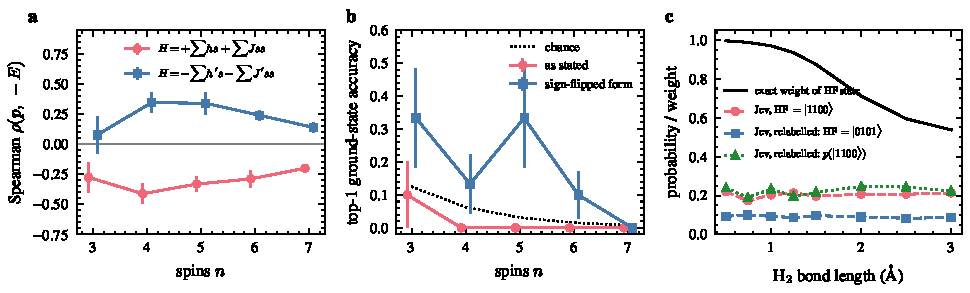
\includegraphics[width=\linewidth]{figs/fig3_hamiltonian.pdf}
\caption{\jev{} given a Hamiltonian in its input (E2). \textbf{a},~Rank correlation between \jev{}'s probability for each spin configuration and its negative energy, for random Ising models as stated (circles) and with the same energies written in the sign-flipped textbook form (squares); mean $\pm$ s.e.m.\ over 10 instances. \textbf{b},~Top-1 ground-state accuracy; dotted line, chance $2^{-n}$. \textbf{c},~Exact weight of the Hartree--Fock state of H$_2$ (STO-3G, Jordan--Wigner) and \jev{}'s probability for it, before and after relabelling the qubits so that the Hartree--Fock state is $|0101\rangle$.}
\label{fig:hamiltonian}
\end{figure}

\subsection{E3: chemistry decisions track the stated stretch factor}

Table~\ref{tab:e3} scores \jev{}'s marginal probabilities against the PySCF labels.
Its rankings are informative (AUROC 0.76, 0.81 and 0.89), but every prompt states the stretch factor, and that number alone ranks multireference character and instability as well or better (0.87 and 0.87; 0.71 for $T_1$); for multireference character \jev{} is worse than the bare stretch factor (difference $-0.16$, 95\% CI $-0.28$ to $-0.02$).
Within the one stretch level where the labels are mixed (1.5 times equilibrium), \jev{}'s AUROC is 0.57, 0.58 and 0.48.
Ablations locate the signal (added after review).
Removing the molecule name changed little (AUROC 0.83, 0.76, 0.90), whereas removing the stretch note while keeping name and geometry dropped \jev{} to 0.57, 0.65 and 0.71, with Brier scores worse than the base rate.
Four rewordings of each question moved AUROC by at most 0.1 and did not change this picture.

\jev{}'s probabilities are also poorly calibrated: its Brier score is much worse than that of a leave-one-molecule-out logistic model on the stretch factor and HOMO--LUMO gap for multireference character and instability, and equal for $T_1$.
Platt recalibration, fitted leave-one-molecule-out, closes the gap for instability and improves $T_1$, but does not help for multireference character.
Used as an extra feature in the logistic model, \jev{} gives small but consistent Brier improvements for $T_1$ ($-0.025$, 95\% CI $-0.038$ to $-0.011$) and for instability ($-0.023$, CI $-0.042$ to $-0.002$), and none for multireference character.
So \jev{} carries a little information beyond two cheap descriptors, but most of what it reports is the stretch factor it was given.

\begin{table}[t]
\centering
\small
\caption{Quantum-chemistry decisions on 48 cases (E3; $T_1$ on 47). All logistic and recalibration models are fitted leave-one-molecule-out. Molecule-clustered 95\% intervals for AUROC are shown in Fig.~\ref{fig:chemistry}a.}
\label{tab:e3}
\begin{tabular}{lcccccc}
\toprule
& \multicolumn{2}{c}{Multireference} & \multicolumn{2}{c}{$T_1>0.02$} & \multicolumn{2}{c}{RHF unstable} \\
\cmidrule(lr){2-3}\cmidrule(lr){4-5}\cmidrule(lr){6-7}
Predictor & AUROC & Brier & AUROC & Brier & AUROC & Brier \\
\midrule
Base rate & -- & 0.236 & -- & 0.234 & -- & 0.182 \\
Stretch factor (stated in prompt) & 0.87 & 0.123 & 0.71 & 0.189 & 0.87 & 0.110 \\
Logistic (stretch, HOMO--LUMO gap) & 0.89 & 0.118 & 0.79 & 0.171 & 0.90 & 0.104 \\
\addlinespace
\jev{} & 0.76 & 0.207 & 0.81 & 0.170 & 0.89 & 0.184 \\
\jev{}, Platt-recalibrated & 0.73 & 0.199 & 0.80 & 0.151 & 0.86 & 0.112 \\
Logistic + \jev{} & 0.86 & 0.128 & 0.79 & 0.146 & 0.93 & 0.082 \\
\addlinespace
\jev{}, name removed & 0.83 & 0.172 & 0.76 & 0.183 & 0.90 & 0.175 \\
\jev{}, stretch note removed & 0.57 & 0.329 & 0.65 & 0.306 & 0.71 & 0.338 \\
\jev{}, geometry only & 0.59 & 0.339 & 0.65 & 0.310 & 0.68 & 0.346 \\
\bottomrule
\end{tabular}

\end{table}

\subsection{E5--E6: a larger molecule set and a routing workflow (added after review)}

To test whether E3 depends on textbook molecules, we repeated it on 31 less common molecules (among them LiF, NaH, MgO, SiS, P$_2$, Be$_2$, O$_3$, FNO, HOF and N$_2$O), each at the same four stretches, with the same prompts and the same labelling protocol.
After excluding cases without a converged RHF, CCSD or singlet CASCI root, 111--114 of the 124 cases remained per label.
The picture is similar (Fig.~\ref{fig:scaleup}a).
\jev{}'s AUROC was 0.81, 0.76 and 0.80, against 0.80, 0.60 and 0.79 for the bare stretch factor and 0.84, 0.68 and 0.85 for the leave-one-molecule-out logistic model; none of the differences from the stretch factor is significant.
With geometry only, AUROC fell to 0.64, 0.54 and 0.56.
Two things differ from the textbook set.
Within a single stretch level \jev{} now separates multireference from single-reference cases (AUROC 0.76--0.90), so on less familiar molecules it draws on more than the stated stretch; and its probabilities are compressed, with the mean $p$(multireference) rising only from 0.42 to 0.58 across stretches while the true rate rises from 0.10 to 0.91.
Adding \jev{} to the logistic model again reduced the Brier score slightly, significantly only for instability ($-0.014$, 95\% CI $-0.024$ to $-0.002$).

For 32 small species with a close singlet--triplet competition (carbenes, silylenes, diatomics such as C$_2$, SiC, BN and O$_2$) we asked for the ground-state multiplicity, with CCSD(T)/cc-pVDZ adiabatic gaps as reference (16 singlets, 16 triplets).
\jev{} was right for 26 of 32 (0.81), close to ordering the states by their Hartree--Fock energies (0.78) and above always answering singlet (0.50); five of its six errors called a singlet a triplet (Fig.~\ref{fig:scaleup}b).

Finally we asked whether \jev{} can route calculations.
For 97 small cases where full CI is affordable (78 in STO-3G, 19 in 6-31G), CCSD(T) missed full CI by more than 1.6~\Eh{} in 38\%.
\jev{}'s probability that CCSD(T) is reliable ranked the failures with AUROC 0.76 (95\% CI 0.65--0.85), against 0.65 for the $T_1$ diagnostic, which needs a CCSD calculation; the difference is not significant (CI $-0.03$ to $0.24$).
At the budget of the $T_1>0.02$ rule, which sends 47\% of cases to a multireference method, \jev{}'s ranking left 11 failures against 12 for $T_1$, but the failures it left were smaller (mean error 2.2 against 10.8~\Eh{}; Fig.~\ref{fig:scaleup}c).
A rule that routes every stretched geometry did better than both, leaving 8 failures while routing 70\% of cases.
\jev{}'s own probabilities cannot set the threshold: they lie between 0.15 and 0.46 while the true reliability rate is 0.62, so ``route if $p<0.5$'' sends every case to the expensive method, and their Brier score (0.358) is worse than the base rate (0.236).

\begin{figure}[t]
\centering
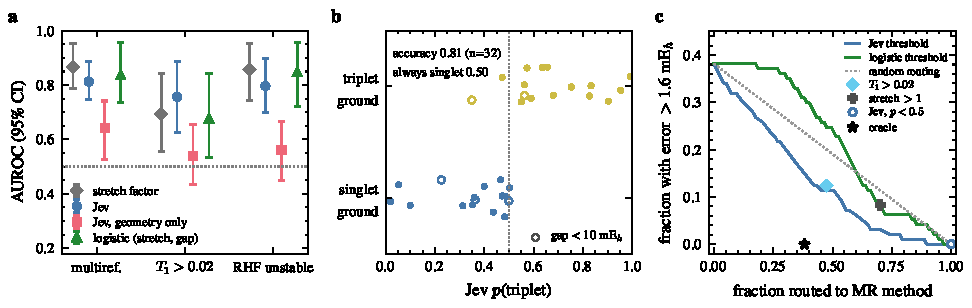
\includegraphics[width=\linewidth]{figs/fig5_scaleup.pdf}
\caption{A larger set and a routing workflow (E5--E6). \textbf{a},~AUROC with molecule-clustered 95\% intervals on 31 less common molecules for the stated stretch factor, \jev{}, \jev{} with geometry only, and a leave-one-molecule-out logistic model. \textbf{b},~\jev{}'s probability of a triplet ground state for 32 species, grouped by the CCSD(T) ground state; open markers have gaps below 10~\Eh{}. \textbf{c},~Fraction of cases whose final error exceeds 1.6~\Eh{} against the fraction routed to a multireference method, for thresholds on \jev{} and on the logistic model, the $T_1$ rule, a stretch rule, \jev{}'s own $p<0.5$ threshold and an oracle.}
\label{fig:scaleup}
\end{figure}

\subsection{E4: determinant ranking for selected CI is a fixed template}

Selected CI keeps only the determinants that matter \citep{huron1973iterative,holmes2016heat}.
For ten systems we built a symmetric active space on stable RHF orbitals (CAS(6e,5o) with 100 determinants for seven systems, 25 determinants for three), gave \jev{} the active orbital energies and the determinant list in occupation notation, and asked which non-reference determinant has the largest weight in the exact ground state.
We added determinants in the resulting order, in spin-complete groups (all determinants with the same spatial occupation), diagonalised the Hamiltonian in each subspace, kept the lowest singlet root, and measured the error against full CASCI.
Comparators were the oracle ordering by exact $|c_i|^2$, the first-order weight $|H_{i0}|^2/(H_{ii}-H_{00})^2$, the Epstein--Nesbet second-order contribution $|H_{i0}|^2/(H_{ii}-H_{00})$ used once, iterative CIPSI, which recomputes that criterion against the current wavefunction after each addition, excitation rank, and random order; all ties were broken at random and averaged over 30 draws.

Averaged over the whole curve, \jev{}'s ordering beats random order in 9 of 10 systems (paired Wilcoxon $p=0.006$) and the excitation-rank rule in 9 of 10 ($p=0.049$), is indistinguishable from the one-shot first- and second-order estimates (6 of 10 each, $p\ge 0.7$), and loses to iterative CIPSI in all ten ($p=0.002$; Fig.~\ref{fig:chemistry}b,c).
The question-aligned metric is less favourable.
\jev{}'s top choice was never the oracle's top determinant: in every system it was the HOMO$\to$LUMO single excitation, which by Brillouin's theorem does not couple to the RHF reference.
Across the seven systems with the same active space, its ranking was nearly identical (median Spearman correlation 0.97 between systems), so \jev{} applies one template to every molecule.
Asking instead one Noul per determinant (``weight above 0.01'') did worse and was indistinguishable from random order (7 of 10, $p=0.43$).

\begin{figure}[t]
\centering
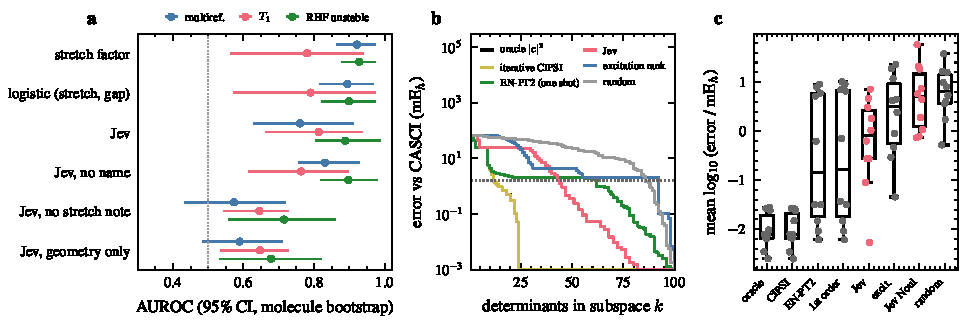
\includegraphics[width=\linewidth]{figs/fig4_chemistry.pdf}
\caption{\jev{} in quantum-chemistry workflows. \textbf{a},~AUROC with 95\% molecule-clustered bootstrap intervals for the three E3 labels, for the stretch factor alone, a logistic model, \jev{}, and three \jev{} input ablations. \textbf{b},~Selected-CI error against subspace size for N$_2$ at equilibrium, CAS(6e,5o)/cc-pVDZ; dotted line, 1.6~\Eh{}. \textbf{c},~Mean $\log_{10}$ error over the whole curve for ten systems; lower is better. ``Jev Noul'' is the per-determinant elicitation.}
\label{fig:chemistry}
\end{figure}

\PH{E7 subsection: open-weight models.}

\section{Discussion}

\jev{}'s outputs can be read as local energies, and within one domain these energies carry an approximate pairwise landscape: the fitted couplings predict answers the fit never saw.
The landscape is not exact.
Asymmetric couplings, violated total probability and unnormalised negations persist under a matched null, under rewording, and in a control where the exact joint is printed in the input.
This is the behaviour one expects when heads are calibrated one at a time \citep{heckerman2000dependency}, since calibrated marginals need not share a joint.
A Gibbs sampler run on such conditionals converges to a distribution that depends on the update order, so there is no single energy whose minima one could search for.
Because \jev{} also adopts stated facts only partially, a cleaner separation of incoherence from soft conditioning would need access that the API does not provide.

Given a Hamiltonian as text, \jev{} does not compute with it.
Its preferences follow the printed signs of the coefficients, reverse when the same energies are printed with opposite signs, and for H$_2$ return the textbook answer even after the qubits are relabelled.
This agrees with the developer's own warning that \jev{} is not a calculator \citep{typesafe2026jaggedness} and with the fragility of language models on numerical reasoning \citep{mirzadeh2024gsm}.
A model that cannot rank the eight configurations of a three-spin Ising model cannot stand in for an annealer or a variational solver \citep{lucas2014ising,peruzzo2014variational}.

For quantum-chemistry decisions, most of \jev{}'s apparent skill came from a stretch factor that we stated, which is the information a chemist would also use, and it vanished when that note was removed.
With the note, \jev{} adds a small, statistically clear amount of information to a two-descriptor model for two of three labels, at a cost of thousandths of a cent per query, which makes it a plausible extra feature in a triage model if it is recalibrated on local data.
It should not be used to rank determinants: its ranking is one template shared across molecules, and iterative CIPSI, which a selected-CI code already runs, is far better.
On less familiar molecules \jev{} did show some discrimination beyond the stretch note, and as a router it ranked CCSD(T) failures at least as well as $T_1$ without any correlated calculation.
Both uses need a threshold chosen on local data, because \jev{}'s own probabilities are compressed toward the middle and shifted, and a plain rule that routes stretched geometries was better still in our set.
\PH{E7 discussion.}

\paragraph{Limitations.}
We studied one model version through a black box, and later versions may behave differently.
Our conditionals are soft, because stated facts are only partly adopted.
The chemistry set is small and made of textbook molecules at uniform stretches, labels depend on thresholds and on the active space, and the selected-CI spaces are far from production scale.
Pairwise and three-way tests cover a small part of the possible coherence conditions, and the three-way test is underpowered.
Two-decimal rounding and sampling noise limit the resolution of every energy we report.

\section{Conclusion}

\jev{}'s typed probabilities can be read as energies that approximately follow one pairwise landscape, but not as a Hamiltonian.
They do not track a physical Hamiltonian supplied in the input, and in chemistry they mostly repeat what the prompt states.
The black-box tests used here, coupling symmetry under a matched null, a stated-joint positive control and held-out prediction from a fitted Ising energy, apply to any model that answers many questions about one input.

\paragraph{Code and data.}
Code, the pre-registered plan, all cached API responses and the PySCF ground truth are at \url{https://github.com/dongzhaohe321418-lab/jev-hamiltonian}.
Every analysis and figure can be regenerated offline from the cache.

\paragraph{Use of AI tools.}
The experiments, analysis code and a first draft of the text were produced with the assistance of an AI coding assistant (Anthropic's Claude). The author directed the study, checked the results against the released data and takes responsibility for the content.

\bibliographystyle{unsrtnat}
\bibliography{refs}

\end{document}
